\section*{Abstract}
\begin{textbf}


This study explores human-plant interaction.
This study has been conducted in order to understand what kind of interaction we have to detect in order to have the best and more natural kind of interaction with plants.
The results will be applied in the Internet of Plants (IoP) project which intends to create a fully connected bio-organ system.
The IoP is looking to reduce the gap between humans and plants by creating a symbiotic relationship between 
nature and technology. We envision a world where our daily objects are responsive.





\end{textbf}

\begin{figure}[ht]
    \centering
    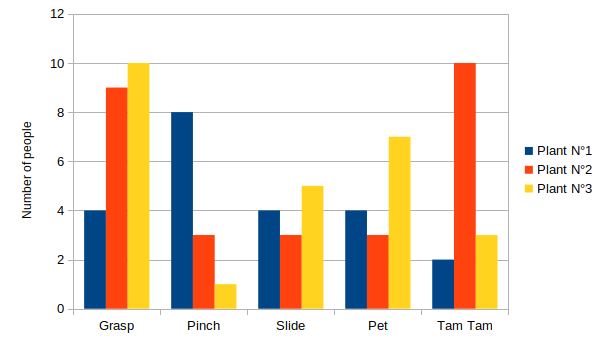
\includegraphics[width=0.42\textwidth]{Images/plant_interaction_chart_1.png}
    \caption{Bar chart that is extracting the main types of interaction regarding each plants.}
    
    \vspace{-0.5cm}
    % \label{fig:setup_user_study}
    \vspace{0.2cm}
\end{figure}

\newpage